\documentclass[aps,twocolumn, floatfix, superscriptaddress]{revtex4}
\usepackage{amsmath, amssymb, amsfonts, gensymb}
\bibliographystyle{apsrev}
\usepackage{graphicx, color, bm}
\graphicspath{ {Figures/} }
\definecolor{r}{rgb}{1,0,0}
\definecolor{b}{rgb}{0,0,1}

%\voffset=1.5 truecm


\begin{document}

\title{Hydrodynamics of a self-propelled camphor boat}

\author{V. S. Akella}
\affiliation{Collective Interactions Unit, OIST Graduate University, 1919-1 Tancha, Onna-son, Okinawa, Japan 904-0495}
\author{D. K. Singh}
\affiliation{Collective Interactions Unit, OIST Graduate University, 1919-1 Tancha, Onna-son, Okinawa, Japan 904-0495}
\author{S. Basu}
\affiliation{Collective Interactions Unit, OIST Graduate University, 1919-1 Tancha, Onna-son, Okinawa, Japan 904-0495}
%\author{V. Churavy}
%\affiliation{Collective Interactions Unit, OIST Graduate University, 1919-1 Tancha, Onna-son, Okinawa, Japan 904-0495}
\author{R. K. Singh}
\affiliation{School of Engineering, Brown University, 182 Hope Street, Providence, RI 02906, USA}
\author{S. Mandre}
\affiliation{School of Engineering, Brown University, 182 Hope Street, Providence, RI 02906, USA}
\author{M. M. Bandi}
\affiliation{Collective Interactions Unit, OIST Graduate University, 1919-1 Tancha, Onna-son, Okinawa, Japan 904-0495}
\email[Corresponding Author: ]{bandi@oist.jp}

\date{\today}

\begin{abstract}
\end{abstract}

%\pacs{}
%\keywords{}

\maketitle
\section{Introduction}
\section{Materials and Methods}
\subsection{Preparation of Cboats}
\label{sec:prep}
The preparation of cboats involves the following steps.
\begin{itemize}
\item Preparation of 5\% w/v agarose (Wako Pure Chemical Industries, Ltd., Cat. No. 346-00072) gel sheets of uniform thickness.
\item Punching out(using Biopunch, Ted Pella, Inc.) discs of agarose gel of required disc diameter. 
\item Soaking the agarose discs in camphoric acid (Wako Pure Chemical Industries, Ltd., Cat. No. 036-01002) saturated methanol (Wako Pure Chemical Industries, Ltd., Cat. No. 138-01836) solution for more than 2 hrs. This process replaces the water from the agarose gel with camphoric acid saturated methanol solution. 
\item Washing and rinsing of the discs in de-ionized water. This step results in the precipitation of camphoric acid in the agarose gel matrix.
\end{itemize}
\subsection{Experimental Set Up}
\label{sec:expset}
\begin{figure}[ht]
    \begin{center}
       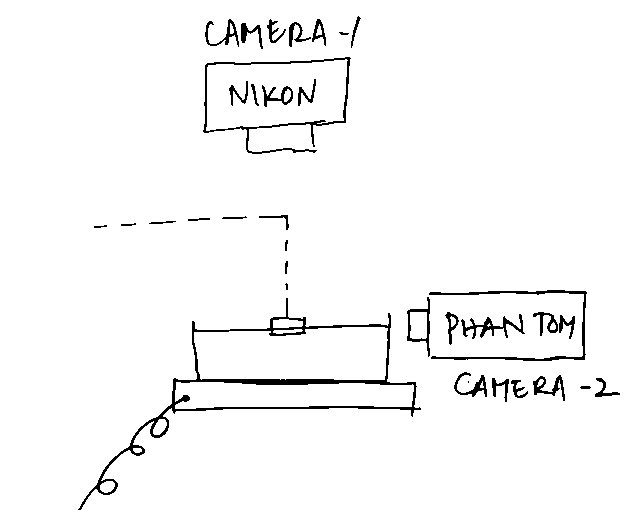
\includegraphics[scale=0.25]{figure1.jpg}
    \end{center}
    \caption{Experimental Set Up.}
    \label{fig:expset}
\end{figure}
The basic experimental set up shown in figure~\ref{fig:expset} involves a glass petri dish (25 mm diameter and 5 cm height) filled with de-ionized water (obtained from Milli-Q Integral Water Purification System with resistivity, $\rho=\mathrm{18\ M} \Omega\ \mathrm{cm}$) up to 4 cm and is illuminated using a light tablet from the bottom. When needed, we used Sodium Dodecyl Sulfate (Wako Pure Chemical Industries, Ltd., Cat. No. 196-08675) to modify the surface tension of water. The camphoric acid spread dynamics are recorded using Phantom v641 Hi-Speed camera at 1000 fps. The cboat dynamics are recorded using Nikon D800E camera at 30 fps. 
\section{Stationary Cboat}
In order to understand the fluid dynamics associated with the motion of cboat at the air-water interface and the fluid directly below, as a first step, we held the cboat fixed at the air-water interface as shown in figure~\ref{fig:expset}. The dynamics at the interface are recorded using camera 1 (figure~\ref{fig:expset}), located directly above the cboat while the dynamics in the bulk are recorded using camera 2 (figure~\ref{fig:expset}), located on the side. For brevity, we discuss our findings in two parts, 1. The transient regime, which is observed from the instance of cboat's contact with the air-water interface until the steady state reached and 2. The steady state regime. 
\subsection{\label{sec:caspread}Transient Regime}
% \label{sec:caspread}
When a drop of surfactant is introduced at the air-water interface, it spreads on the interface to minimize the interfacial free energy. The surfactant front emanates radially outwards until the interface is saturated with the surfactant and radius of the surfctant front(Jensen, Mahesh) is given by the following equation.
\begin{equation} \label{eq:jensen}
r(t) \approx \left(\frac{\Delta \gamma}{\mu \rho}\right)^{1/4} t^{3/4}
\end{equation}
where, $\Delta \gamma$ is the Harkins spreading co-efficient, $\mu$ is the dynamic viscosity of the fluid and $\rho$  is the density of the fluid.  
\begin{figure}[ht]
    \begin{center}
       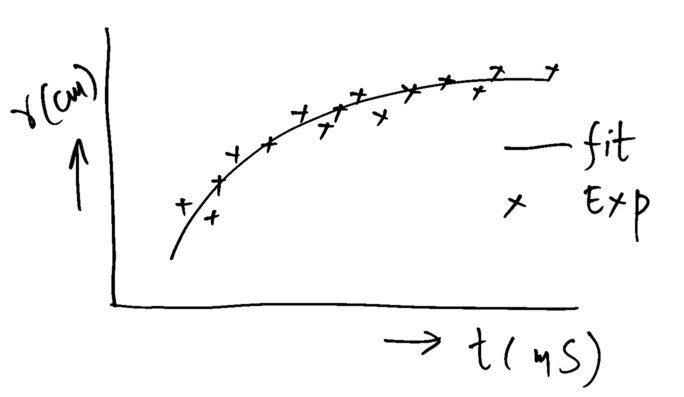
\includegraphics[scale=0.25]{figure2.jpg}
    \end{center}
    \caption{Camphoric acid radial spread vs. time}
    \label{fig:caspread}
\end{figure}
The surfactant front is visualized using hydrophilic tracer particles sparsely sprinkled on the air-water interface. The measured radius of the surfactant front as a function of time is shown in figure~\ref{fig:caspread}. As mentioned earlier, camphoric acid being mildly surface active behaves like a surfactant. Furthermore, camphoric acid is a van der Waals' solid and camphoric acid molecules sublime into the surroundings. This additional physics results in a different functional form for the radially emanating surfactant front than equation~\ref{eq:jensen}. In this article, we obtained an analytical form for the radius of the surfactant front using a simplistic model (Appendix ??) and is given by,
\begin{equation} \label{eq:shreyas}
r(t) \approx r_{\infty} \left(1-\mathrm{e}^{-t/\tau} \right)
\end{equation}
Figure~\ref{fig:caspread} shows the experimental data for the radius of the surfactant front and the fit using the above model. The steady state value of $r(t)$ is the maximum distance, measured from the center of the cboat, to which camphoric acid spreads without subliming/evaporating. As expected, when the sublimation/evaporation rate, $k\to0$ equation~\ref{eq:shreyas} reduces to equation~\ref{eq:jensen}.

\subsection{Steady State Regime}
\label{sec:steady}
In the steady state, there is a balance between the flux of camphoric acid molecules entering the air-water interface (due to Interfacial tension forces drawing the camphoric acid molecules out of the cboat to minimize the interfacial free energy) and camphoric acid molecules leaving air-water interface (due to sublimation/evaporation). As discussed in section~\ref{sec:caspread}, typically the system reaches a steady state in less than a second. We recorded the steady state dynamics in the fluid directly below the cboat using camera 2. We held the cboat fixed and performed Particle Image Velocimetry (PIV) in the fluid directly below the cboat. From the PIV data, we obtained the fluid velocity at the air-water interface and below it. We also calculated the Blasius boundary layer thickness as a function of the radial distance, measured from the center of the cboat. Furthermore, we used the measured fluid velocity to calculate the steady state concentration profile of the camphoric acid around the cboat using the following equation. 
\begin{equation} \label{eq:advdiff}
\frac{\partial}{\partial t} c(\vec{x}, t) - \mathrm{D} \nabla^2 c(\vec{x}, t) + \vec{u}.\vec{\nabla} c(\vec{x}, t) + k c(\vec{x}, t) = 0 
\end{equation}
Where, the first and second terms describe the diffusion of camphor acid, third term describes the advection of camphoric acid due to the fluid flow and the last term describes the sublimation/evaporation of camphoric acid into the surroundings. Note that, the complete theoretical description of the system involves solving equation~\ref{eq:advdiff} coupled with Navier-Stokes’ equation. However, we simplified the system by measuring the fluid velocity, $\vec{u}$. In a steady state,
\begin{equation} \label{eq:steady}
\mathrm{D} \nabla^2 c(\vec{x}) - \vec{u}.\vec{\nabla} c(\vec{x}) - k c(\vec{x}) = 0 
\end{equation}
Substituting typical values for $D$ and $\vec{u}$ we note that, $\mathrm{D} \frac{d^2}{d x^2} c(\vec{x}) \ll u \frac{d}{dx}c(\vec{x})$ . Hence, in 1D, the equation reduces to the following.
\begin{equation} 
\frac{d}{dx}c(x) = -\frac{k}{u}c(x)
\end{equation}
Solving the above equation yields, 
\begin{equation} \label{eq:approx1d}
c(x) = \exp\left(-\frac{k}{u}x\right) + \mathrm{const.}
\end{equation}
From the measured values of velocity, $\vec{u}$, we calculated the expected concentration profile, shown in figure~\ref{fig:blandca}, around the cboat. 
\begin{figure}[ht]
    \begin{center}
       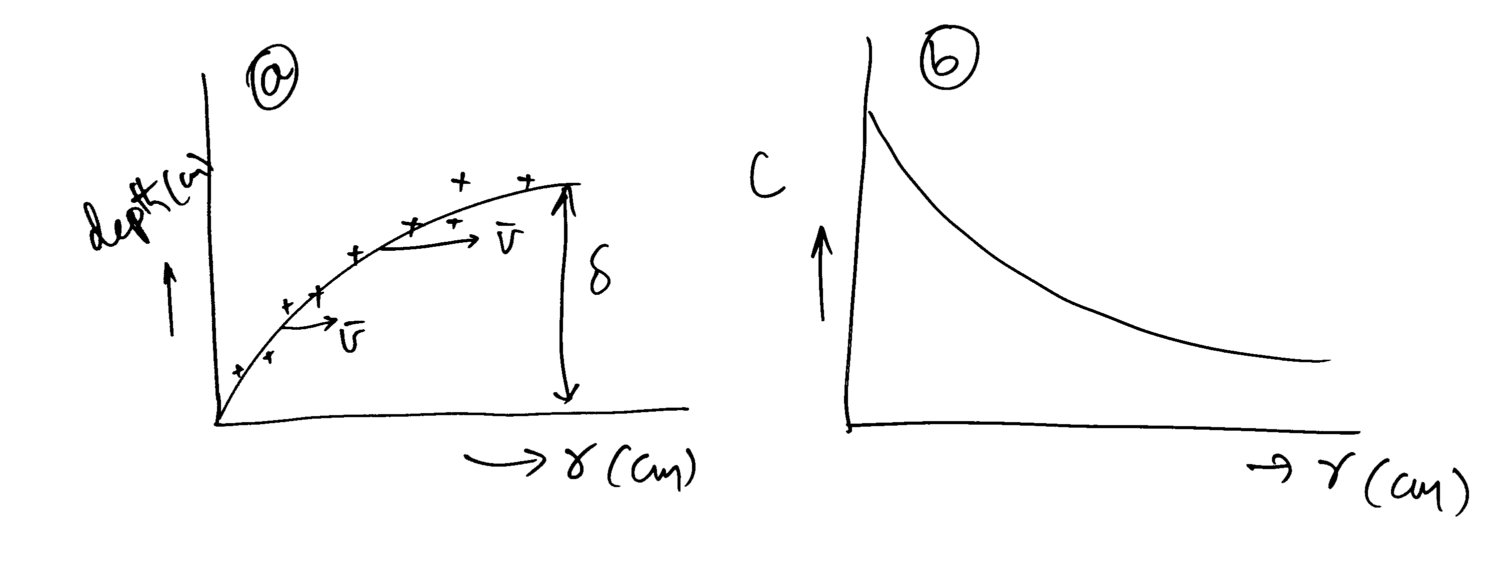
\includegraphics[scale=0.18]{figure3.jpg}
    \end{center}
    \caption{(a) Experimentally measured Blasius layer depth (b) Calculated camphoric acid concentration profile.}
    \label{fig:blandca}
\end{figure}
\section{Dynamic Cboat}
When the cboat is placed at the air-water interface, the following processes lead to the movement of cboat on the air-water interface.
\begin{itemize}
\item Camphoric acid spreads onto the air-water interface via two processes. 1. Interfacial forces draw the camphoric acid molecules out of the cboat to minimize the interfacial energy. 2. Diffusion of camphoric acid molecules onto the air-water interface. Dissolution is another mechanism by which camphoric acid is drawn out of cboat but it is very minimal as the solubility of camphoric acid is $\approx$ 40 mM at 25 \celsius.
\item As mentioned earlier, camphoric acid is a surface active molecule and lowers the air-water interfacial energy. When a cboat is introduced at the air-water interface, the out-flux of camphoric acid molecules from the cboat sets up interfacial tension gradients symmetrically around the cboat. A random perturbation arising due to change in local temperature or contamination of air-water interface due to unavoidable dust particles in air spontaneously break the symmetric interfacial tension gradients around the cboat. When the perturbation is strong enough to overcome the viscous drag forces on the cboat, the cboat starts moving. Once the cboat starts moving it further enhances the asymmetry resulting in continuous motion of the cboat.
\item The air-water interface never gets saturated with the camphoric acid because camphoric acid sublimes into room. Therefore the motion of the cboat lasts as long as there is camphoric acid in the cboat.
\end{itemize}
\subsection{Lifetime of a Cboat}
\label{sec:lifetime}
The forces acting on the cboat are, 1. Marangoni forces set up by the interfacial tension gradients which are in turn caused camphoric acid concentration gradients, 2. Drag forces due to the viscosity of the medium. During the course of the experiment, camphoric acid sublimes into the surroundings resulting in decrease in Marangoni forces. Another mechanism that affects the lifetime of a cboat is: the dissolution of camphoric acid in water which decreases the background air-water interfacial tension resulting in lesser interfacial tension gradients. However, the amount of camphoric acid in a cboat ($\simeq 7\ \mathrm{mg}$) is negligibly small to modify the interfacial tension of water by a measurable amount. The interfacial tension of water, when saturated with camphoric acid ($\simeq 8\ \mathrm{g/l}$), is $\simeq 60\ \mathrm{dy/cm}$. As camphoric acid sublimes the physical characteristics of the system change continuously. Figure~\ref{fig:lifetime} is the speed of a cboat as function of time. 
\begin{figure}[ht]
    \begin{center}
       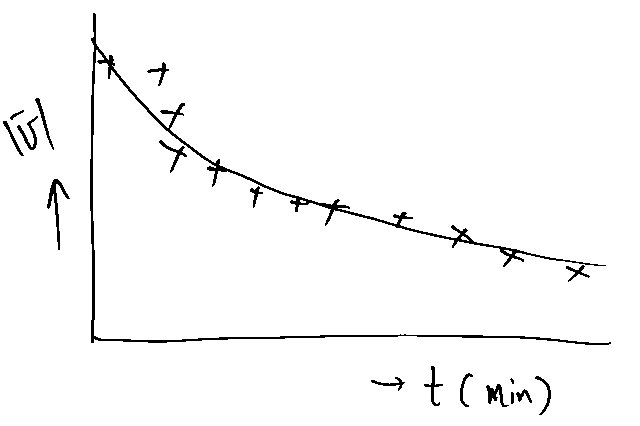
\includegraphics[scale=0.25]{figure4.jpg}
    \end{center}
    \caption{Lifetime of the Cboat.}
    \label{fig:lifetime}
\end{figure}
\subsection{Oscillatory Motion of the Cboat}
\label{sec:movingcboat}
Another interesting phenomenon observed in cboat dynamics is the oscillatory motion of the cboat. Figure~\ref{fig:absvnosds} shows the time traces of the cboat speed at different intervals and the corresponding power spectra. At the beginning of the experiment there is a strong peak at $\approx 1\ \mathrm{Hz}$ in the power spectrum. However the peak completely disappears at long times. The observed phenomenon is shown in figure~\ref{fig:absvnosds}.   
\begin{figure}[ht]
    \begin{center}
       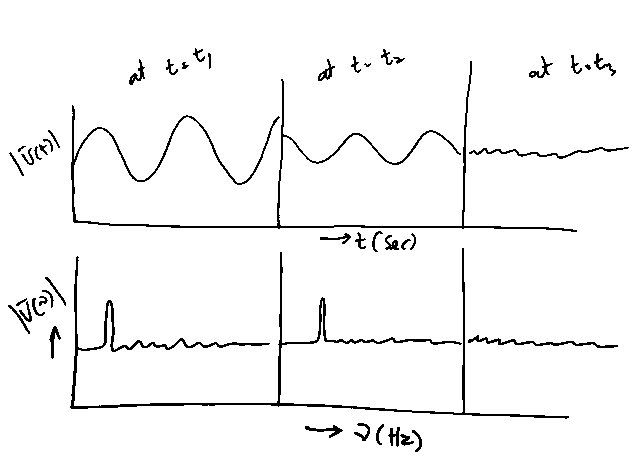
\includegraphics[scale=0.35]{figure5.jpg}
    \end{center}
    \caption{(a) Oscillation in speed of the cboat at different intervals. (b) The power spectrum of speed.}
    \label{fig:absvnosds}
\end{figure}
The motion of cboat involves two processes. 1. At an instant position of the cboat on the air-water interface, Marangoni forces are established because camphoric acid spreads and creates interfacial tension gradients around the cboat and 2. The Marangoni forces propel the cboat to a new position where the interfacial tension (concentration of camphoric acid) is high (low). At the new position, the same processes repeat and the cboat continues to move. Let us define $\tau_{\gamma}$ as the time required to establish sufficient Marangoni forces to overcome the drag forces and $\tau_{\lambda} = \frac{\|\vec{u}\|}{\lambda}$ as the time required for the cboat to move a distance, $\lambda$ defined as the maximum distance, measured from the center of the cboat, to which camphoric acid spreads without subliming/evaporating. The cboat motion can be continous, oscillatory or intermittent when $\tau_{\gamma} < \tau_{\lambda}$, $\tau_{\gamma} \approx \tau_{\lambda}$ or $\tau_{\gamma} > \tau_{\lambda}$ respectively. From the measurements in section~\ref{sec:caspread}, the radius of influence of the cboat is $\approx 3.6\ \mathrm{cm}$ for a 3 $\mathrm{mm}$ diameter cboat. Furthermore, the average distance travelled by the cboat during a period of oscillation ($\approx 1\ \mathrm{Hz}$) is also $\approx$ 3.6 $\mathrm{cm}$. This observation indicates that, the cboat always moves from one position to another position in steps of $\lambda$ however, the motion appears to be continuous, oscillatory or intermittent depending on $\tau_{\gamma}$ and $\tau_{\lambda}$. A typical cboat dynamics experiment, with a 3 $\mathrm{mm}$ diameter cboat, is recorded for 20 minutes during which we observed the oscillatory and continuous motions as shown in figure~\ref{fig:absvnosds}. During the course of the experiment, camphoric acid sublimes into the surroundings resulting in continuous decrease in $\lambda$ of the cboat, thereby increasing $\tau_{\lambda}$. Therefore, the transistion from $\tau_{\gamma} \approx \tau_{\lambda}$ to $\tau_{\gamma} < \tau_{\lambda}$ leads to oscillatory to continuous motion of the cboat. Further, to experimentally verify the above hypothesis we used Sodium Dodecyl Sulfate (SDS) to modify the interfacial tension of air-water interface. From equation~\ref{eq:jensen}, modifying the background interfacial tension slows down rate of camphoric acid spread on the air-water interfaction thereby increasing $\tau_{\gamma}$. When the interfacial tension is sufficiently modified, the system goes into $\tau_{\gamma} > \tau_{\lambda}$ regime exhibiting the intermittent motion of the cboat. Figure~\ref{fig:absvsds} shows the intermittent, oscillatory and continuous regimes at different concentrations of SDS.
\begin{figure}[ht]
    \begin{center}
       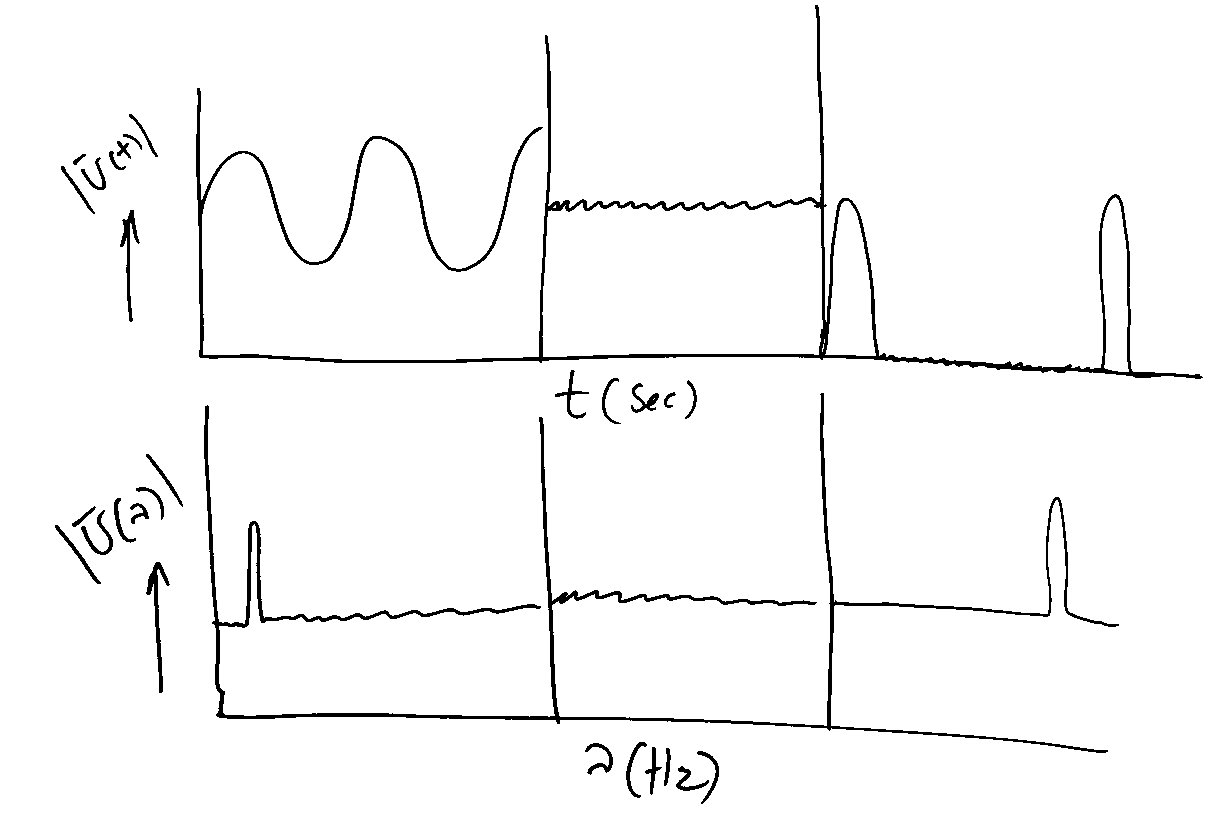
\includegraphics[scale=0.2]{figure6.jpg}
    \end{center}
    \caption{(a) Oscillations in the speed of the cboat at different concentrations of Sodium Dodecyl Sulfate (SDS) (b) The power spectrum of speed.}
    \label{fig:absvsds}
\end{figure}
% \section{Discussion}
\section{Summary}
\label{sec:summary}

%Figures:
%Fig1a: Schematic of exp. setup.
%Fig1b: fixed camphor boat with radial circle of camphor spread
%Fig1c: Moving CBoat (maybe trajectory with cboat at end of trajectory)

%Fig2a: Short-time transient Rs(t) vs. t

%Fig3a: Rs(t) vs t for long time transient
%Fig3b: |v(t) vs t for lifetime of experiment

%Fig4a: Schematic for Saikat's model
%Fig4b: Convection PIV snapshot

%Fig5a: speed vs. time (steady-state)
%Fig5b: Speed power spectrum (2Hz oscillation peak)
%Fig5c: Speed power spectrum with SDS.

%\begin{figure}
%\begin{center}
%\includegraphics[width = 2.75 in]{}
%\end{center}
%\caption{}
%\label{fig1}
%\end{figure}


\acknowledgments
VSA, DKS, SB and MMB were supported by the OIST Graduate University with subsidy funding from the Cabinet Office, Government of Japan. RKS was hosted by OIST Graduate University on a research internship while performing this work. MMB acknowledges L. Mahadevan for introducing the camphor boat system and subsequent scientific discussions, and D. Vu Anh for help with preliminary experiments.

\bibliography{all}

\end{document} 
